\documentclass[times, utf8, diplomski, numeric]{fer}
\usepackage[utf8]{inputenc}
\usepackage[T1]{fontenc}
\usepackage{currvita}
\usepackage{graphicx}
\usepackage{epstopdf}
\usepackage{listings}
\usepackage{textcomp}
\usepackage{booktabs}
\usepackage{algorithmic}
\usepackage{algorithm}
\usepackage{xfrac}
\usepackage[bookmarks]{hyperref}
\usepackage{color}

% koristimo zadebljane vektore, a ne strelice
\renewcommand{\vec}[1]{\mathbf{#1}}

% TODO komanda koja u PDFu daje crveni, kapitalizirani, bold text
\newcommand\todo[1]{\colorbox{yellow}{\textcolor{red}{#1}}}

% ovo je za numeriranje samo jedne linije unutar align okoline
\newcommand\numberthis{\addtocounter{equation}{1}\tag{\theequation}}

% definicija jezika koji nema nista, pa se nista ne naglasava
% koristi se za troadresni kod, ispise tokena i slicno
\lstdefinelanguage{blank}{
	sensitive=false, 
	morecomment=[l]{;},
}

% neke boje koje koristimo u formatiranju ispisa
\usepackage{color}
\definecolor{mygreen}{rgb}{0,0.6,0}
\definecolor{mylightgray}{rgb}{0.95,0.95,0.95}

% definicija formatiranja ispisa, ponesto promjenjena u odnosu na pretpostavljenu
\lstset{ %
  backgroundcolor=\color{mylightgray},   % choose the background color; you must add \usepackage{color} or \usepackage{xcolor}
  basicstyle=\footnotesize\ttfamily,        % the size of the fonts that are used for the code
  breakatwhitespace=false,         % sets if automatic breaks should only happen at whitespace
  breaklines=true,                 % sets automatic line breaking
  captionpos=b,                    % sets the caption-position to bottom
  commentstyle=\color{mygreen},    % comment style
  deletekeywords={...},            % if you want to delete keywords from the given language
  escapeinside={\%*}{*)},          % if you want to add LaTeX within your code
  extendedchars=true,              % lets you use non-ASCII characters; for 8-bits encodings only, does not work with UTF-8
  frame=none,                    % adds a frame around the code
  keepspaces=true,                 % keeps spaces in text, useful for keeping indentation of code (possibly needs columns=flexible)
  keywordstyle=\color{blue},       % keyword style
  language=c,           	       % the language of the code
  morekeywords={*,...},            % if you want to add more keywords to the set
  numbers=none,                    % where to put the line-numbers; possible values are (none, left, right)
  numbersep=5pt,                   % how far the line-numbers are from the code
  numberstyle=\tiny\color{gray}, % the style that is used for the line-numbers
  rulecolor=\color{black},         % if not set, the frame-color may be changed on line-breaks within not-black text (e.g. comments (green here))
  showspaces=false,                % show spaces everywhere adding particular underscores; it overrides 'showstringspaces'
  showstringspaces=false,          % underline spaces within strings only
  showtabs=false,                  % show tabs within strings adding particular underscores
  stepnumber=2,                    % the step between two line-numbers. If it's 1, each line will be numbered
  stringstyle=\color{red},     % string literal style
  tabsize=2,                       % sets default tabsize to 2 spaces
  title=\lstname                   % show the filename of files included with \lstinputlisting; also try caption instead of title
}

\begin{document}

\title{Jezični model temeljen na neuronskoj mreži}
\thesisnumber{1095}

\author{Florijan Stamenković}

\maketitle

\tableofcontents

\chapter{Uvod}

Tema ovog diplomskog rada je jezični model baziran na umjetnoj neuronskoj mreži. Jezični model je računalni sustav korišten u području obrade prirodnog jezika (statističke lingvistike) koji nalazi primjenu primjerice u automatiziranom prevođenju, prepoznavanju govora, i mnogim drugim zadatcima obrade teksta. Umjetne neuronske mreže koriste se kao jedan od pristupa izradi prediktivnih modela koji je u posljednjih desetak godina sve popularniji, zahvaljujući novim tehnikama i odličnim rezultatima. Kako bi se jezični model temeljen na neuronskoj mreži razmotrio u širem kontekstu, u ovom radu je implementirano nekoliko pristupa izgradnji jezičnih modela.

Naglasak je stavljen na objašnjenje kako prediktivne modele koristiti za izgradnju jezičnih modela. Objašnjavaju se prednosti i nedostatci isprobanih pristupa, kao i izazovi implementacije. Modeli su definirani matematički egzaktno, ali se ne ulazi u detalje računalne implementacije pošto su za to dostupni brojni kvalitetni materijali. Pretpostavlja se da čitatelj posjeduje osnovno znanje iz područja strojnog učenja, neuronskih mreža i linearne algebre. Ovaj rad na temelju tih znanja čitatelju može razjasniti osnovne pojmove o izradi i primjeni jezičnih modela, kao i specifičnosti, prednosti i nedostatke razmatranih modela. Bitno je naglasiti da su u ovom radu obrađeni tek neki od brojnih pristupa izradi jezičnih modela, rad nipošto nije iscrpan.

Rad je organiziran na sljedeći način. U drugom poglavlju ("Jezični model") se govori o jezičnim modelima općenito. Razmatra se njihova svrha, moguće primjene, te se iskazuje najčešće korištena matematička definicija jezičnog modela. Sljedeća četiri poglavlja razlažu pristupe izgradnji jezičnog modela koji su razmotreni u ovom radu. U svakom od tih poglavlja je matematički definiran po jedan model. Komentirani su pristupi implementaciji, ali algoritmi treniranja i korištenja nisu ispisani. Za svaki od modela se razmatraju prednosti i nedostatci. Potom je u sedmom poglavlju ("Vrednovanje") opisan način usporedbe jezičnih modela općenito, kao i konkretno vrednovanje provedeno u ovom radu. Razmotreni su rezultati vrednovanja kako bi čitatelj stekao što bolji dojam o primjenjivosti korištenih modela. U konačnici slijede zaključak i reference.


\chapter{Jezični model}
\label{sec:jezicni_modeli}

Jezični model jedan je od ključnih elemenata računalnog procesiranja prirodnog jezika. Glavni zadatak tom računalnom sustavu je ocjenjivanje pripadnosti teksta u prirodni jezik za koji je sustav rađen. Dodatno, poželjno je da sustav između više ponuđenih može izabrati tekst koji je najviše "u duhu" jezika. Primjerice, model hrvatskog jezika trebao bi biti sposoban ocijeniti da je niz \textit{"dan je lijep"} generalno više u duhu jezika od \textit{"lijepo dana biti"}, a da niz \textit{"it's a nice day"} u dotični jezik ne pripada.

Smislenost niza riječi može se promatrati iz pravopisne, gramatičke i semantičke perspektive. Model treba biti sposoban nizu \textit{"lijep dan"} dati bolju ocjenu nego nizu \textit{"ljep dan"}, jer je drugi niz pravopisno neispravan. Model treba bolje ocijeniti niz \textit{"lijep dan"} od niza \textit{"lijepo dani"}, po kriteriju gramatičke ispravnosti. Konačno, treba bolje ocijeniti niz \textit{"lijep dan"} od niza \textit{"gumeni parket vječno"}, jer je drugi niz semantički skoro sasvim besmislen.

\section{Primjena}

Jezični modeli imaju velik broj primjena. Sustavi za strojno prevođenje koriste ih kako bi odabrali što smisleniji među više potencijalnih prijevoda. Sustavi za prepoznavanje govora koriste ih kako bi prepoznate slogove i riječi pretvorili u konačni tekst. Sustavi za pretraživanje teksta mogu ih koristiti za mjerenje sličnosti između termina pretrage i dokumenta. Ovo su samo neke od mnogih primjena, povećanjem dostupne količine informacija i mogućnosti njihove računalne obrade, moguće primjene i kvaliteta jezičnih modela imaju trend povećanja.

\section{Probabilistička definicija}

Pošto prirodni jezik omogućava praktično neiscrpne mogućnosti kombiniranja riječi u tekst, smisleno je jezični model razmatrati statistički. Na temelju nekog korpusa teksta moguće je napraviti sustav koji za proizvoljni niz označava koliko je sličan tekstu iz korpusa. Ovo je u skladu s definicijom i iskazanim svojstvima jezičnog modela. Kako bi se računalni statistički sustav izgradio, potrebno je smislenost teksta definirati probabilistički.

Razmatra se niz riječi $w_1, w_2, ... , w_m$. Niz sadrži $m$ riječi, pri čemu $w_i$ označava riječ koja se pojavljuje na $i$-tom mjestu u nizu. Primjerice, za niz \textit{"Nebo je plavo"}, pojedine riječi se označavaju na sljedeći način: $w_1="Nebo"$, $w_2="je"$, $w_3="plavo"$. U kontekstu statističkog modeliranja jezika potrebno je definirati vjerojatnost pojavljivanja proizvoljnog niza riječi. Oznaka za vjerojatnost niza riječi slijedi.

\[
P(\text{niz}) = P(w_1, w_2, ... , w_m)
\]

Dakle, razmatra se vjerojatnost da se pojavio niz od $m$ riječi, pri čemu je prva riječ niza $w_1$, sljedeća $w_2$, i tako sve do konačne riječi niza $w_m$. U skladu s teorijom vjerojatnost, izraz za vjerojatnost niza moguće je faktorizirati (izraziti kao umnožak jednostavnije definiranih vjerojatnosti) na sljedeći način.

\begin{align*}
P(w_1, w_2, ... , w_m)
  &= P(w_1) P(w_2 | w_1) P(w_3 | w_1, w_2) ... P(w_m | w_1, w_2, ... , w_{m - 1 }) \\
  &= \prod_{i = 1}^m{P(w_i|w_1, ... , w_{i - 1})}
\end{align*}

Pri tome je $P(w_i | w_1, ... , w_{i - 1})$ uvjetna vjerojatnost pojavljivanja riječi $w_i$ na $i$-toj poziciji u nizu, ako su joj prethodile riječi $w_1$, ... $w_{i - 1}$ na pozicijama $1$, ... , $i - 1$. Primjetimo kako je ovakva faktorizacija u skladu sa čovjekovim čitanjem teksta (slijedno po riječima).

Slijedi primjer izraza vjerojatnosti i faktorizacije, za već spomenuti niz \textit{"Nebo je plavo"}.

\begin{align*}
P(\textit{"Nebo je plavo"})
  = &P(w_1=\textit{"Nebo"}, w_2=\textit{"je"}, w_3=\textit{"plavo"}) \\
  = &P(w_1=\textit{"Nebo"}) P(w_2=\textit{"je"} | w_1=\textit{"Nebo"}) \\
  &P(w_3=\textit{"plavo"} | w_1=\textit{"Nebo"}, w_2=\textit{"je"})
\end{align*}

Česće se u literaturi može vidjeti kraći zapis iste faktorizacije.

\begin{align*}
P(\textit{"Nebo je plavo"})
  = &P(\textit{"Nebo"}, \textit{"je"}, \textit{"plavo"}) \\
  = &P(\textit{"Nebo"}) P(\textit{"je"} | \textit{"Nebo"}) P(\textit{"plavo"} | \textit{"Nebo"}, \textit{"je"})
\end{align*}

Iako egzaktna, iskazana faktorizacija vjerojatnosti niza praktična za dugačke nizove jer je vjerojatnost riječi na poziciji $i$ uvjetovana svim prethodnim riječima. Stoga se u jezičnim modelima najčešće koristi kontekst ograničene duljine od $n$ riječi. Primjerice, za kontektst duljine $n = 3$, svaka riječ se razmatra samo s obzirom na prethodne dvije.

\begin{align*}
P(w_1, w_2, ... , w_m)
  &\approx P(w_1) P(w_2 | w_1) P(w_3 | w_1, w_2)  ... P(w_m | w_{m - 2}, w_{m - 1}) \\
  &\approx \prod_{i = 1}^m{P(w_i | w_{i - 2}, w_{i - 1})}
\end{align*}

Općenito, za proizvoljnu duljinu konteksta \textit{n} faktorizacija je sljedeća.

\begin{align*}
P(w_1, w_2, ... , w_m)
  &\approx P(w_1) P(w_2 | w_1) P(w_3 | w_1, w_2)  ... P(w_m | w_{m - (n - 1)}, ... , w_{m - 1}) \\
  &\approx \prod_{i = 1}^m{P(w_i | w_{i - (n - 1)}, ... , w_{i - 1})}
\end{align*}

Tako definiran jezični model više nije probabilistični egzaktan, ali se može praktično implementirati kao računalni sustav.

U kontekstu obrade prirodnog jezika, standardna oznaka za niz od \textit{n} riječi je "\textit{n}-gram". Za $n=1, 2, 3$ govorimo o "unigramu", "bigramu", odnosno "trigramu", dok za $n=4$ o "4-gramu" itd. U tom smislu niz \textit{"Nebo je plavo"} sadrži unigrame \{\textit{"Nebo"}, \textit{"je"}, \textit{"plavo"}\}, bigrame \{\textit{"Nebo je"}, \textit{"je plavo"}\} i trigram \{\textit{"Nebo je plavo"}\}.

Kada se koristi ograničeni kontekst, javlja se pitanje optimalne duljine konteksta, odnosno vrijednost parametra $n$. Pošto na konačno značenje niza mogu utjecati riječi koje su od promatrane riječi proizvoljno daleko, može se pretpostaviti da je veći kontekst bolji od manjeg. Iako ovo u idealnom slučaju vrijedi, u praksi se koriste relativno male duljine konteksta. Razlog za to je rijetkost pojavljivanja dugih nizova. Vjerojatnost pojavljivanja nekog konkretnog niza riječi duljine $n$ drastično pada kako $n$ raste. Istovremeno, jezični model se bazira na nekom konkretnom korpusu koji ima konačnu količinu teksta. Čak i ako je korpus vrlo velik (što je poželjno), vjerojatnost pojavljivanja nekon proizvoljnog, smislenog niza duljine primjerice 100 je vrlo mala. U drugu ruku, ako je korpus dovoljno velik, smislene kombinacije od tri ili četiri riječi pojavit će se često. Stoga je moguće napraviti sustav koji na temelju statistike pojavljivanja trigrama ili 4-grama vrednuje smislenost neviđenog teksta, ali je praktički nemoguće napraviti sustav koji bi to činio na temelju pojavljivanja 100-grama. U praksi se stoga često koriste konteksti duljine oko četiri riječi, ovisno o primjeni. Neke implementacije modela baziranih na velikom korpusu teksta mogu povećati kontekst do desetak riječi, rijetko više od toga. 

Alternativni pristup ograničavanju veličine konteksta je kompresija odnosno aproksimacija konteksta veće (ponekad pune) duljine. Konkretno, ako kontekst prikažemo kao funkciju prethodnih riječi, moguća je sljedeća faktorizacija.

\begin{align*}
P(w_1, w_2, ... , w_m)
  &\approx P(w_1) P(w_2 | f(w_1)) P(w_3 | f(w_1, w_2)) ... P(w_m | f(w_1, w_2, ... , w_{n - 1 })) \\
  &\approx \prod_{i = 1}^n{P(w_i | f(w_1, ... , w_{i - 1}))}
\end{align*}

Pri tome funkcija $f(...)$ preslikava kontekst proizvoljne duljine u zapis fiksne duljine. Ovakva formulacija koristi se primjerice u izvedbi jezičnih modela korištenjem rekurzivnih neuronskih mreža. Pošto se u ovom radu ne koriste implementacije bazirane na toj formulaciji, onoe se neće u nastavku spominjati.

Postoje varijante jezičnih modela koje kao kontekst ne promatraju riječi koje doslovno prethode promatranoj, već riječi iz šire okoline. Jasno je da su takvi modeli primjenjvi samo u situacijama kada je cijeli niz poznat unaprijed, ali takve situacije su dovoljno česte da bi dotični modeli bili primjenjivi. Neki modeli čak razmatraju "koncepte", uzorke sačinjene od nekoliko specifičnih riječi koje se mogu pojaviti bilo gdje u tekstu. Ovakvi modeli se neće razmatrati u nastavku.

Konačno, bitno je spomenuti jezične modele bazirane na manjim lingvističkim jedinicama. Jezični modeli bazirani na morfemima i znakovima su od nedavno, pogotovo sa sve većom primjenom dubokih neuronskih mreža, postali uspooredivi i čak u nekim primjenama bolji od leksičkih modela CITAT.

\section{Načini izvedbe}

Postoje brojne implementacije jezičnih modela. Većina njih izvedena je iz probabilističke formulacije modela, ili tu formulaciju aproksimiraju. Tehnike korištene za izradu modela variraju. U ovom diplomskom radu biti će uspoređene izvedbe prebrojavanjem \textit{n}-grama, jezični model temeljen na jednostavnoj neuronskoj mreži i log-bilinearni probabilistički model. Njihova definicija i opis slijede.

\chapter{Prebrojavanje \textit{n}-grama}

Najjednostavniji pristup implementaciji jezičnog modela bazira se na prebrojavanju odnosno frekvenciji pojavljivanja \textit{n}-grama. Na primjeru trigrama, vjerojatnost pojavljivanja riječi $w_i$ na $i$-tom mjestu u tekstu je sljedeća.

\[
P(w_i | w_{i - 2}, w_{i - 1}) = \frac{C(w_{i - 2}, w_{i - 1}, w_i)}{C(w_{i - 2}, w_{i - 1})}
\]

Pri tome je $C(w_a, ... , w_b)$ funkcija prebrojavanja koja za niz $w_a, ... , w_b$ daje broj njegovih pojavljivanja u korpusu teksta nad kojim se model gradi. Uvjetna vjerojatnost pojavljivanja riječi, s obzirom na prethodne dvije, je dakle broj pojavljivanja relevantnog trigrama, podjeljeno s brojem pojavljivanja bigrama koji joj prethode. 

Intuicija je sljedeća. Ako se u korpusu za učenje jezičnog modela trigram \textit{"dan je lijep"} pojavljuje 10 puta, a bigram \textit{"dan je"} 42 puta, tada je vjerojatnost da se nakon konteksta \textit{"dan je"} pojavi riječ \textit{"lijep"} jednaka $P("lijep" | "dan", "je") = 10 / 42$.

Ovako definiran procijenitelj vjerojatnosti zapravo je procijenitelj  najveće izglednosti (ML-procijenitelj, engl.\ \textit{maximum likelihood}). Općenito razmatranje statističkih procjenitelja je izvan opsega ovog diplomskog rada, više informacija na temu može se naći u materijalima na temu statistike i strojnog učenja.

Definirana je uvjetna vjerojatnost za kontekst duljine $n = 3$. Formulaciju je potrebno poopćiti na proizvoljnu vrijednost parametra $n$. Uvjetna vjerojatnost riječi s obzirom na kontekst proizvoljne duljine $n$ je sljedeća.

\begin{equation}
\label{eq:ngram_freq}
P(w_i | w_{i - (n - 1)}, ... , w_{i - 1}) = \frac{C(w_{i - (n - 1)}, ... , w_{i - 1}, w_i)}{C(w_{i - (n - 1)}, ... , w_{i - 1})}
\end{equation}

\section{Zaglađivanje}

Već je spomenuto kako je otežavajuć faktor izgradnje jezičnih modela rijetkost pojavljivanja duljih \textit{n}-grama u konačnom korpusu teksta. Ovaj problem zapravo nije ograničen samo na modele koji koriste veliki kontekst. Čak i za male vrijednost $n$, primjerice 3, lako se može desiti da neki smisleni trigram ne bude prisutan u korpusu na kojem se model bazira. Ovo nije začuđujuće, s obzirom da je broj mogućih trigrama $|V|^3$, gdje je $V$ skup svih riječi jezika (vokabular) za koji se model gradi. Primjerice, za engleski se jezik procjenjuje da sadrži oko $300,000$ riječi\footnote{Oxford English Dictionary, http://www.oed.com}, što znači da je broj mogućih trigrama oko $27 \cdot 10^{15}$. Jasno je da se mnogi smisleni trigrami među njima nikada ne pojavljuju u korpusu za učenje, bez obzira na njegovu veličinu. U slučaju da se pri korištenju modela evaluira vjerojatnost jednog od njh, po definiciji \ref{eq_ngram_freq} ona će biti 0. Numerički i intuitivno vjerojatnost 0 govori kako je nešto nemoguće, što se svakako želi izbjeći, pogotovo ako se radi smislenom \textit{n}-gramu.

 U jezičnim modelima koji se temelje na prebrojavanju \textit{n}-grama se problem rijetkosti rješava zaglađivanjem \engl{smoothing}. Ideja je da se u račun vjerojatnosti unese pretpostavka kako je korpus na kojem se model bazira samo uzorak jezika. Pretpostavivši da postoje mnogi \textit{n}-grami koji nisu prisutni u korpusu, ali zavređuju određenu vjerojatnost, njen račun se modificira kako bi se vjerojatnosna masa šire rasporedila. Time se disproporcije u vjerojatnostima \textit{n}-grama smanjuju, odnosno zaglađuju.

Postoji više pristupa zaglađivanju, neki od popularnijih su aditivno (Laplace), Good-Turing i Knesser-Ney zaglađivanje. Aditivno zaglađivanje u pravilu daje lošije rezultate, koristi se pretežno u edukativne svrhe. Zaglađi vanje Kneser-Ney metodom je manje intuitivno, ali daje odlične rezultate. U ovom radu implementirano je aditivno zaglađivanje i zaglađivanje Kneser-Ney metodom.

\subsection{Aditivno zaglađivanje}

Ideja aditivnog zaglađivanja CITAT je da se svakom mogućem \textit{n}-gramu pridjeli neka mala vjerojatnost, makar se taj \textit{n}-gram nije pojavio u korpusu za treniranje. U izrazu vjerojatnosti mora se voditi računa da suma vjerojatnosti svih mogućih \textit{n}-grama bude 1. Uzevši to u obzir dobiva se sljedeći izraz uvjetne vjerojatnosti riječi.

\[
P(w_i | w_{i - (n - 1)}, ... , w_{i - 1}) = \frac{C(w_{i - (n - 1)}, ... , w_{i - 1}, w_i) + \alpha}{C(w_{i - (n - 1)}, ... , w_{i - 1}) + \alpha d}
\]

Pri tome je $\alpha$ proizvoljan broj, tipično 1 ili manje, a $d$ broj svih mogućih \textit{n}-grama. Koristeći aditivno zaglađivanje na jednostavan se način izbjegava da vjerojatnost bilo kojeg \textit{n}-grama bude 0. Nedostatak ovog pristupa je to što svim \textit{n}-gramima umjetno povećava broj pojavljivanja za isti broj $\alpha$, bez obzira na njihovu relativnu smislenost. Modificiranjem vjerojatnosti kvalitetnijim pretpostavkama drugi oblici zaglađivanja u pravilu postižu bolje rezultate.

\subsection{Zaglađivanje Kneser-Ney metodom}

Prezentirano u radu CITAT, zaglađivanje Kneser-Ney metodom jedan je od načina zaglađivanja oduzimanjem fiksne vrijednost od vjerojatnosti \textit{n}-grama \engl{absolute value discounting}. Ideja je da se oduzimanjem od vjerojatnosti \textit{n}-grama dobije "višak" vjerojatnosne mase, koja se potom raspodjeljuje svim \textit{n}-gramima, uključujući one manje zapostavljene u korpusu za treniranje. Generiranje viška vjerojatnosne mase, na primjeru trigrama, se u Kneser-Ney metodi vrši na sljedeći način.

\[
P(w_i | w_{i - 2}, w_{i - 1}) =
  \frac{max\left(C(w_{i - 2}, w_{i - 1}, w_i) - \delta, 0\right)}
    {C(w_{i - 2}, w_{i - 1})} + ...
\]

Pri tome je $\delta$ vrijednost koja se oduzima od prebrojavanja, u rasponu $\delta \in (0, 1)$. S obzirom da nije dozvoljeno da vjerojatnost postane negativna, potrebno je koristiti funkciju $max(x, 0)$, za slučaj kada je $C(w_{i - 2}, w_{i - 1}, w_i) < \delta$, odnosno kada je $C(...) = 0$. 

Dobiveni višak vjerojatnosne mase Kneser-Ney metoda raspodjeljuje na temelju prebrojavanja \textit{n}-grama nižeg reda (manjeg parametra \textit{n}). Stoga, u slučaju kada se model bazira na trigramima, izraz se nastavlja dodavanjem vjerojatnosti bazirane na bigramima.

\[
P(w_i | w_{i - 2}, w_{i - 1}) =
  \frac{max\left(C(w_{i - 2}, w_{i - 1}, w_i) - \delta, 0\right)}
    {C(w_{i - 2}, w_{i - 1})} + \lambda P(w_i | w_{i - 1})
\]

Pri tome je $\lambda$ višak vjerojatnosti dobiven oduzimanjem fiksne vrijednosti $\delta$. Moglo bi se učiniti kako je $\lambda = \delta$, pošto je upravo $\delta$ količina oduzete vjerojatnosti, ali to bi bilo pogrešno. Količina $\delta$ je oduzeta samo u slučajevima kada je $C(w_{i - 2}, w_{i - 1}, w_i) >= 1$. U suprotnom, kada je $C(...) = 0$, funkcija $max(x, 0)$ poništava to oduzimanje. Broj slučajeva kada se oduzimanje provelo je broj slučajeva kada je $C(w_{i - 2}, w_{i - 1}, w_i) >= 1$. Stoga je $\lambda$ definiran na sljedeći način.

\[
\lambda = \left|\{w : C(w_{i - 2}, w_{i - 1}, w) > 0\}\right| \frac{\delta}{C(w_{i - 2}, w_{i - 1})} 
\]

Prvi dio izraza (sve što prethodi razlomku) prestavlja broj slučajeva kada se oduzimanje provelo. Konkretno, definiran je skup riječi $w$ za koje je broj pojavljivanja trigrama $C(w_{i - 2}, w_{i - 1}, w)$ veći od $0$ (što povlači da se oduzimanje provodi), te je potom uzeta veličina tog skupa, odnosno broj provedenih oduzimanja. Drugi dio izraza sačinjen je od razlomka. U brojniku je $\delta$, što broj provedenih oduzimanja pretvara u konkretnu vrijednost svih oduzimanja. Nazivnik je isti kao u osnovnom izrazu prebrojavanja, kako bi vjerojatnost ostala normalizirana na sumu od 1.

Time je objašnjeno kako se u zaglađvanju Kneser-Ney metodom dio vjerojatnosne mase prenosi na \textit{n}-grame nižeg reda, ali stvar tu ne završava. Kako bi se kvaliteta zaglađivanja dodatno poboljšala, procijena vjerojatnosti \textit{n}-grama nižeg reda bazirana je na "vjerojatnosti nastavljanja" \engl{continuation probability}. Pitanje koje vjerojatnost nastavljanja formulira je sljedeće: koliko je vjerojatno da se riječ $w$ pojavila nakon prethodnih, bez obzira kojih? Odnosno, koliko je riječ $w$ dobar "nastavljač"? Ta vjerojatnost smatra se proporcionalnom broju različitih prehodnih konteksta nakon kojih se pojavljuje.

Intuicija vjerojatnosti nastavljanja se često objašnjava na primjeru bigrama \textit{"San Francisco"}. Pretpostavivši da se u korpusu teksta taj bigram pojavljuje često, vjerojatnost unigrama \textit{"Francisco"} biti će proporcionalno velika, ali je njena vjerojatnost nastavljanja mala jer se javlja isključivo nakon riječi \textit{"San"}. Ako je na temelju tog korpusa potrebno dovršiti rečenicu \textit{"Cipele popravlja \_."}, jednostavan model bi mogao na temelju vjerojatnosti unigrama preferirati riječ \textit{"Francisco"}, jer se riječ \textit{"postolar"} u korpusu pojavljuje rijeđe. Kneser-Ney metoda korištenjem vjerojatnosti nastavljanja ne preferira riječ \textit{"Francisco"}, koja se javlja isključivo nakon riječi \textit{"San"}, jer se riječ \textit{"postolar"} javlja kao nastavak većeg broja riječi, iako je u korpusu rjeđa.

Matematički, vjerojatnost nastavljanja bigrama $P_{\text{cont}}$ definirana je na sljedeći način.

\[
P_{\text{cont}}(w_i | w_{i - 1}) =
  \frac{\left|\{w_{i - 1} : C(w_{i - 1}, w_i) > 0\}\right|}
  {\sum_{w_j \in V}\left|\{w_{j - 1} : C(w_{j - 1}, w_j) > 0\}\right|}
\]

U brojniku se nalazi broj različitih riječi nakon koji se javlja $w_i$. Na temelju bigrama \textit{"San Francisco"}, za riječ \textit{"Francisco"} će brojnik biti samo 1. Za riječ \textit{"postolar"} će brojnik biti veći, jer se ta riječ javlja kao nastavak većeg broj riječi, primjerice u \textit{"dobar postolar"} i \textit{"otac mu je postolar"}. U nazivniku se nalazi normalizacijska suma koja je jednaka za obje riječi iz primjera.

Zaglađivanje Kneser-Ney metodom se koristi tako da se za \textit{n}-grame najvišeg reda koriste obične vjerojatnosti bazirane na prebrojavanju, od kojih se oduzimaju fiksne vrijednosti. Dobivenom se dodaje vjerojatnost nastavljanja \textit{n}-grama jednog reda niže, množeno faktorom $\lambda$. Pri tome se vjerojatnost nastavljanja isto tako zaglađuje Kneser-Ney metodom, čime je definirana rekurzivna jednadžba. Vjerojatnost najnižeg reda (unigrama), procjenjuje se njihovom frekvencijom. Rekurzivno definirano zaglađivanje Kneser-Ney metodom moguće je koristiti za proizvoljnu duljinu konteksta $n$.

\section{Implementacija}

Praktična izvedba prebrojavanja \textit{n}-grama je konceptualno vrlo jednostavna. Tekst treba pretvoriti u \textit{n}-grame i za svaki \textit{n}-gram ustanoviti broj pojavljivanja u korpusu. Kompleksnije metode zaglađivanja, poput Kneser-Ney metode, koriste dodatna prebrojavanja koja su tek nešto kompliciranija za izvedbu. Nakon što se shvati što je točno potrebno prebrojati, implementacija algoritma nije zahtjevna. Jedini problem prebrojavanja \textit{n}-grama je njihova brojnost.

Već je spomenuto kako je za engleski jezik broj mogućih trigrama okvirno $27 \cdot 10^{15}$. Za pohranu broja pojavljivanja svakog od njih korištenjem samo dva okteta računalne memorije bilo bi potrebno oko 50 tisuća \textit{terabyte}-a memorije. Očigledno je ovo sa današnjim računalima neizvedivo. Problem je potrebno rješiti drukčije. Mora se uzeti u obzir da je većina tih trigrama iznimno malo vjerojatno, te se oni nikada ne javljaju u tekstu. Stoga je nepotrebno trošiti memoriju na njih. Zato se za pohranu broja pojavljivanja \textit{n}-grama koriste rijetke \engl{sparse} podatkovne strukture. Pamte se brojevi pojavljivanja samo onih \textit{n}-grama koji su se barem jednom pojavili. Ovaj pristup rješava problem memorijske zahtjevnosti, ali je izvedba kompliciranija. Rijetke strukture podataka mogu se implementirati na različite načine, o čemu im ovise memorijske i brzinske performanse. Kvalitetno upoznavanje rijetkih struktura podataka preporučeno je pri pokušaju implementacije jezičnih modela baziranih na prebrojavanju \textit{n-grama}.

\chapter{Neuronska mreža}

Umjetne neuronske mreže jedan su od često korištenih pristupa izgradnje prediktivnih modela. Osnove korištenja neuronskih mreža ovdje neće biti razjašnjene, kao uvod u to područje može se konzultirati CITAT.

Jezični model može se smatrati svojevrsnim klasifikatorom. Za viđeni kontekst, model treba predvidjeti sljedeću riječ. Ako je kontekst baziran na \textit{n}-gramima, model na temelju ($n - 1$) prethodne riječi treba predvidjeti sljedeću. Ovakva interpretacija jezičnog modela jednostavno se preslika u umjetnu neuronsku mrežu, koje se često koriste za klasifikaciju. Nadalje, pošto u prirodnom jeziku više različitih riječi može opravdano slijediti nekom prethodnom kontekstu, pogodno je mrežu definirati kao "meki" klasifikator koji ne predviđa točno koja riječ slijedi, već daje vjerojatnosnu ocjenu svim riječima vokabulara.

\section{Ulaz u mrežu}
\label{sec:lnnet_input}
Neuronske mreže kao ulaznu vrijednost primaju vektor varijabli koje mogu biti binarne, cijeli ili realni brojevi. Postavlja se pitanje kako predočiti riječ kao vektor brojeva koji se mogu dati na ulaz mreže. Riječ je jedan element skupa vokabulara. U tom smislu se svaka riječ može predočiti kao binarni vektor veličine jednake vokabularu, pri čemu su sve vrijednosti vektora $0$, osim one koja odgovara riječi koju vektor prestavlja, koja ima vrijednost $1$. Ovakav zapis jednog elementa skupa se često naziva \textit{"one-hot encoding"}.

Postoji nekoliko problema s ovakvom definicijom neuronskog modela jezika. Veličina ulaznog vektora ovisi o veličini vokabulara i veličini konteksta. S obzirom na to da vokabular može sadržavati desetke tisuća riječi, ulaz u mrežu neminovno bi bio ogroman, što implicira velik broj parametara mreže, dugo treniranje i potrebu za ogromnim skupom za učenje. Nadalje, u ovakvoj definiciji u mreži ne postoji veza između sličnih riječi, pošto je svaka riječ interpretirana kao nezavisan element vokabulara. U tom smislu se riječ \textit{"automobil"} smatra jednako različitom od riječi \textit{"motocikl"} i \textit{"leptir"}, što za jezični model nije pogodno. Poželjno je da jezični model sadrži znanje o sličnosti riječi jer to povećava njegovu sposobnost generaliziranja. Ako je model uspješno naučio u kojim kontekstima se javlja riječ \textit{"automobil"}, poželjno je da u sličnim kontekstima smatra pojavljivanje riječi \textit{"motocikl"} vjerojatnijim od pojavljivanja riječi \textit{"leptir"}.

Navedeni problemi prisutni su i u drugim područjima obrade prirodnog jezika, primjerice u pretraživanju. Česti pristup rješavanju ovog problema je korištenje \textit{"distribuiranih reprezentacija"} riječi CITAT. U ovom pristupu se svaka riječ predočava vektorom realnih brojeva. Ovisno o primjeni vektor može imati nekoliko desetaka do nekoliko stotina elemenata. Dvije su poželjne posljedice korištenja ovog pristupa. Prvo, veličina reprezentacije riječi ne ovisi linearno o veličini vokabulara. Drugo, slične riječi imaju slične distribuirane reprezentacije. Obje posljedice vrlo su pogodne za izgradnju neuronskog jezičnog modela, ali problem sada postaje pronalazak prikladnih distribuiranih reprezentacija svih riječi.

Distribuirane reprezentacije moguće je izgraditi korištenjem latentne semantičke analize CITAT, koja se bazira na linearnoj dekompoziciji matrice pojavljivanja riječi unutar nekog niza. LSA se uspješno koristi za pretraživanje teksta, gdje je za termin pretrage potrebno pronaći relevantne dokumente. Problem pri korištenju LSA pristupa je memorijska zahtjevnost linearne dekompozicije s obzirom na količinu primjera koji se obrađuju. Kako se jezični modeli grade korištenjem što većeg korpusa, LSA nije prikladan alata. Reprezentacije je također moguće izgraditi korištenjem neuronskih mreža specijaliziranih za to CITAT Word2Vec. S obzirom na iterativnu prirodu učenja neuronskih mreža, memorijska složenost lakše se kontrolira. Konačno, moguće je učenje reprezentacija ugraditi u neuronsku mrežu koja ima neku drugu primjenu. Ovaj pristup korišten je u ovom radu.

\section{Definicija mreže}

Neuronski jezični model definiran je na sljedeći način. Ulazni sloj mreže sastoji se od $(n - 1) d$ neurona, pri čemu je $d$ veličina distribuirane reprezentacije riječi. Vrijednosti koje se dovode na ulaz mreže su riječi \textit{n}-grama koje prethode posljednjoj, uvjetovanoj riječi. Mreža nema skrivenih slojeva. Izlaz mreže ima $|V|$ neuronapri čemu svaki neuron predstavlja jednu riječ vokabulara. Izlazni sloj definiran je kao \textit{softmax} sloj. U tom smislu je izlaz mreže vjerojatnosna distribucija posljednje riječi \textit{n}-grama, s obzirom na prethodnih $(n - 1)$ riječi. Slijedi matematična definicija opisane mreže.

\begin{equation}
\label{eq:lnnet}
\begin{split}
P(w_i | w_{i - (n - 1)}, ... , w_{i - 1}) 
  & = \text{softmax}_{w_i}(d(w_{i - (n - 1)}, ... , w_{i - 1}) W + b) \\
  & = \frac{\exp(d(w_{i - (n - 1)}, ... , w_{i - 1}) W_{w_i} + b_{w_i})}
           {\sum_{w \in V} \exp(d(w_{i - (n - 1)}, ... , w_{i - 1}) W_{w} + b_{w})}
\end{split}
\end{equation}

Pri tome $W$ označava matricu težina \engl{weight} mreže između $(n - 1)$ reprezentacije na ulazu i izlaznog sloja, dimenzija $(n - 1) d \times |V|$, dok $W_w$ označava vektor težina mreže između $(n - 1)$ reprezentacije na ulazu i izlaznog neurona za riječ $w$. Funkcija $d(...)$ preslikava slijed riječi $w \in V$ u vektor njihovih distribuiranih reprezentacija, a $b$ označava pristranosti \engl{bias} svih neurona izlaznog sloja, dok $b_w$ označava pristranost neurona izlaznog sloja koji odgovara riječi $w$. Funkciju $d(...)$ isto tako se može definirati kao matričnu operaciju.

\begin{equation}
\label{eq:d_func}
d(w_1, ..., w_k) = \left[R_{w_1}, ..., R_{w_k}\right]
\end{equation}

Pri čemu je $R$ matrica distribuiranih reprezentacija \engl{representation} riječi dimenzija $|V| \times d$, a $R_w$ odgovara retku te matrice koji sadrži reprezentaciju riječi $w$. Može se primjetiti kako se za sve ulazne riječi koristi ista matrica distribuiranih vektora. Time se smanjuje broj parametara mreže i pospješuje učenje reprezentacija (riječi sličnog značenja dobivaju slične reprezentacije).

Mreža je prikazana na slici \ref{fig:nnet}.

\begin{figure}[!htb]
\centering
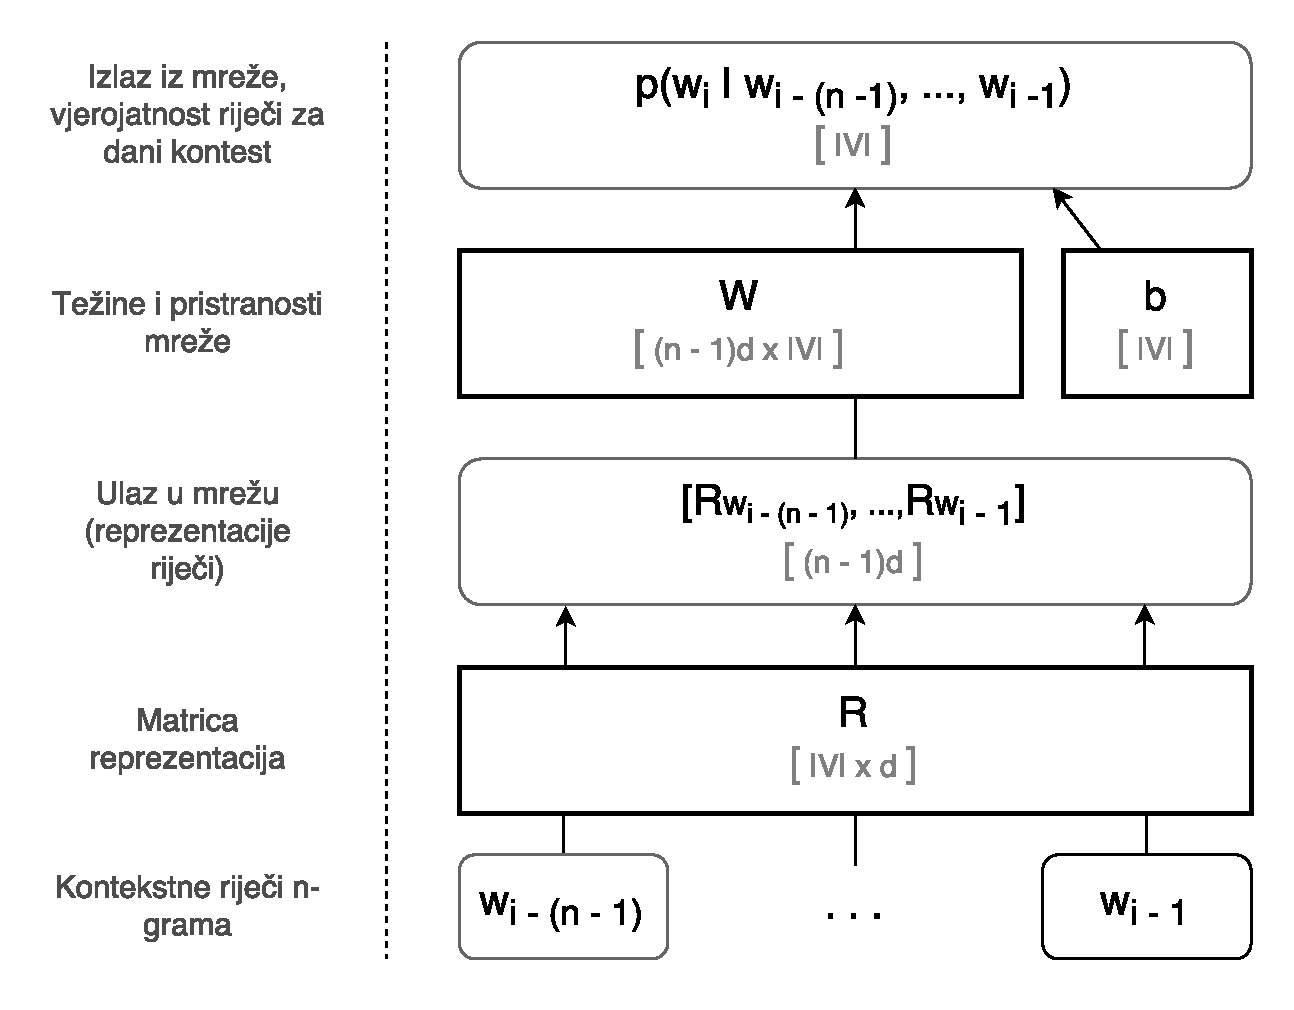
\includegraphics{fig/nnet.pdf}
\caption{Arhitektura neuronskog jezičnog modela. Pravokutnici s debljim rubovima su parametri mreže. Pravokutnici sa zaobljenim rubovima su podatci koji kroz mrežu prolaze.}
\label{fig:nnet}
\end{figure}

\section{Učenje}

Mreža korištena kao model jezika tipična je unaprijedna slojevita neuronska mreža. Mreže tog tipa treniraju se korištenjem algoritma propagacije greške unatrag \engl{backpropagation algorithm}. Gradijentnim spustom se smanjuje greška na skupu za treniranje. Osnove gradijentnog spusta i algoritma propagacije greške unatrag neće biti opisane u ovom radu. Informacije na tu temu su široko dostupne, primjerice u CITAT - Čupić NENR.

Eventualna specifičnost neuronskog modela jezika, u odnosu na standardne unaprijedne slojevite mreže, je korištenje matrice reprezentacija $R$. Odabir retka matrice (što čini funkcija $d(...)$) nije standardna derivabilana matematička operacija. U tom smislu može se postaviti pitanje kako matricu $R$ optimirati gradijentnim spustom. Rješenje leži u tome da se matrica zapravo ne optimira u cjelosti, već se pri svakom podešavanju parametara mreže tijekom rada algoritma propagacije greške unatrag mjenjaju vrijednosti onih distribuiranih reprezentacija koje su u tom koraku korištene. Konkretno, reprezentacija riječi koje su bile na ulazu u mrežu.

\subsection{Smanjenje greške gradijentnim spustom}
\label{sec:nnet_grad}

Algoritam propagacije greške unatrag bazira se na gradijentnom spustu s obzirom na funkciju greške mreže. U originalu se greška minimizirala iterativno koristeći gradijent izračunat na cijelom skupu za učenje. Ovo se naziva grupno \engl{batch} učenje. U praksi se pokazalo kako je efikasnije podijeliti skup za učenje na manje grupe, odnosno mini-grupe \engl{minibatch} i koristiti njih za gradijentni spust. Korištenjem mini-grupa se parametri modela podešavaju češće, što ubrzava učenje. Istovremeno, gradijent nije isti za svaku mini-grupu, što povećava otpornost na zaglavljivanje gradijentnog spusta u lokalnim minimumima. Ekstrem korištenja mini-grupa je podešavanje parametara mreže nakon evaluacije samo jednog primjera za učenje, što se naziva pojedinačno \engl{online} učenje. Ovaj ekstremni pristup rezultira nestabilnim gradijentom, zbog čega se mora smanjiti stopa učenja, i manjom efikasnošću korištenja računalnih resursa uslijed otežane paralelizacije. Stoga se najčešće koriste mini-grupe. Konkretna veličina mini-grupe ovisi domeni primjene, arhitekturi mreže i načinu učenja. Ne postoji univerzalno prikladna veličina.

Osim "običnog" gradijentnog spusta, postoje i modificirane inačice. One parametre mreže ne mjenjaju samo izravno za veličinu negativnog gradijenta pomnoženog stopom učenja, već gradijent ili stopu učenja modificiraju. Najjednostavniji primjer modifikacije gradijenta je korištenje "momenta", pri čemu se čuva informacija o prethodnim iznosima gradijenta, akumulirana u "moment" (analogno momentu kretanja kuglice određene mase koja se kotrlja u smjeru nagiba, ali i u smjeru trenutne brzine). Postoje mnoge inačice gradijentnog spusta. U ovom radu korištena je inačica "RMSprop" \engl{resilient mean square propagation}, opisana u CITAT.

\section{Složenost mreže}

Pri izgradnji jezičnog modela potrebno je voditi račun o memorijskoj i vremenskoj složenosti izrade modela zbog veličine vokabulara koji se u jeziku koristi. U neuronskim mrežama je složenost treniranja usko vezana uz broj slobodnih parametara mreže. Stoga je potrebno vidjeti u kakvoj su vezi parametri jezičnog modela i neuronske mreže.

Matrica distribuiranih reprezentacija $R$ sadrži $|V| d$ parametara, matrica težina $W$ sadrži $(n - 1) d |V|$ parametara, a vektor pristranosti $|V|$ parametara. Sveukupno, mreža sadrži $(n d + 1) |V|$ parametara. Njena memorijska složenost stoga je $O(n d |V|)$. Vremenska složenost treniranja neuronske mreže ovisi o mnogim čimbenicima, ali se u ovom slučaju zbog jednostavnosti mreže može aproksimirati kao $O(n d |V|)$.

\section{Implementacija}

Za implementacije neuronskih mreža dostupni su mnogi alati. Većina njih je visoko optimizirana kako bi što učinkovitije koristili dostupne računalne resurse. Višeprocesorska i višejezgrena računala koriste se za paralelizaciju treniranja mreže, a sve dostupnija je i podrška za treniranje mreža koristeći visoki stupanj paralelizma grafičkih procesora. Nadalje, alati često podržavaju definiciju mreže na visokom stupnju apstrakcije i automatizirani izračun gradijenata, što olakšava implementaciju i smanjuje količinu grešaka u programskom kodu.

U ovom radu za korištena je \textit{open-source} knjižnica Theano\footnote{http://deeplearning.net/software/theano/}, čije sučelje je dostupno za jezik Python\footnote{https://www.python.org/}. Odabrana je zbog fleksibilnosti definiranja modela (lako se koristi s visoke razine apstrakcije, ali omogućava i rad na nižim razinama), automatiziranog izračuna gradijenata i mogućnosti izvršvanja istog koda na centralnim i grafičkim procesorima.

\chapter{Log-bilinearni model}

U radu CITAT 3-new-models-Mnih predložene su tri implementacije jezičnih modela. Najuspješniji među njima je log-bilinearni model.

Log-linearni prediktivni modeli CITAT su klasa modela u kojima je vjerojatnost uzorka proporcionalna eksponenciranoj linearnoj funkciji. Jednostavan primjer takvog modela je već korištena \textit{softmax} funkcija. Prikladni su za modeliranje vjerojatnosti jer eksponencijalna funkcija preslikava iz domene $\mathbb{R}$ u domenu $\mathbb{R}_{\leq 0}$, koja se lako normalizira u vjerojatnosni prostor. Istovremeno, logaritmiranje takve funkcije rezultira linearnom funkcijom (otkud ime "log-linearni modeli"), koja je pogodna za analizu i optimizaciju. Više informacija na temu log-linearnih modela može se naći u literaturi iz područja strojnog učenja CITAT.

Bilinearna funkcija je funkcija dvije varijable koja je s obzirom na njih obje linearna CITAT. U skladu s tim, log-bilinearni probabilistički model definira vjerojatnost proporcionalnu eksponenciranoj bilinearnoj funkciji.

\[
P(a, b) \propto \exp(f_{lin}(a, b))
\]

\section{Log-bilinearni jezični model}

Log-bilinearna funkcija može se primjeniti za definiciju uvjetne vjerojatnosti riječi u jezičnom modelu s obzirom na kontekst. Razmatranja o načinu predstavljanja riječi iz poglavlja \ref{sec:lnnet_input} o neuronskom jezičnom modelu vrijede i za log-bilinearni model. Stoga se i u ovom modelu koriste distribuirane reprezentacije. Za kontekst definiran preko \textit{n}-grama, kakav je i dosad korišten u ovom radu, uvjetna vjerojatnost riječi ima sljedeći oblik.

\begin{equation}
P(w_i | w_{i - (n - 1)}, ... , w_{i - 1}) 
  \propto \exp(d(w_{i - (n - 1)}, ... , w_{i - 1}) W d(w_i)^T + b_{w_i})
\end{equation}

Funkcija $d(...)$ definirana je izrazom \ref{eq:d_func}. $W$ označava matricu preslikavanja $(n - 1)$ $d$-dimenzionalne reprezentacije na ulazu u jedan $d$-dimenzionalni vektor. Nakon što je time ulazni vektor reprezentacija reduciran na $d$ dimenzija, računa se skalarni produkt s reprezentacijom uvjetovan riječi, te se dodaje pristranost za tu riječ. Dobiveni rezultat potrebno je normalizirati u distribuciju vjerojatnosti nad svim riječima vokabulara.

\begin{equation}
P(w_i | w_{i - (n - 1)}, ... , w_{i - 1}) 
  = \frac{\exp(d(w_{i - (n - 1)}, ... , w_{i - 1}) W d(w_i)^T + b_{w_i})}
  {\sum_{w \in V} \exp(d(w_{i - (n - 1)}, ... , w_{i - 1}) W d(w)^T + b_{w})}
\end{equation}

Iako je ova definicija vrlo slična matematičkoj definiciji neuronskog modela jezika \ref{eq:lnnet}, zapravo se ne radi o mreži. Umjesto da se na temelju ulaznih riječi (konteksta) računa funkcija izlaza za $|V|$ izlaznih neurona, računa se mjera podudarnosti sa svakom riječi vokabulara.

Log-bilinearni model je prikazan na slici \ref{fig:lbl}.

\begin{figure}[!htb]
\centering
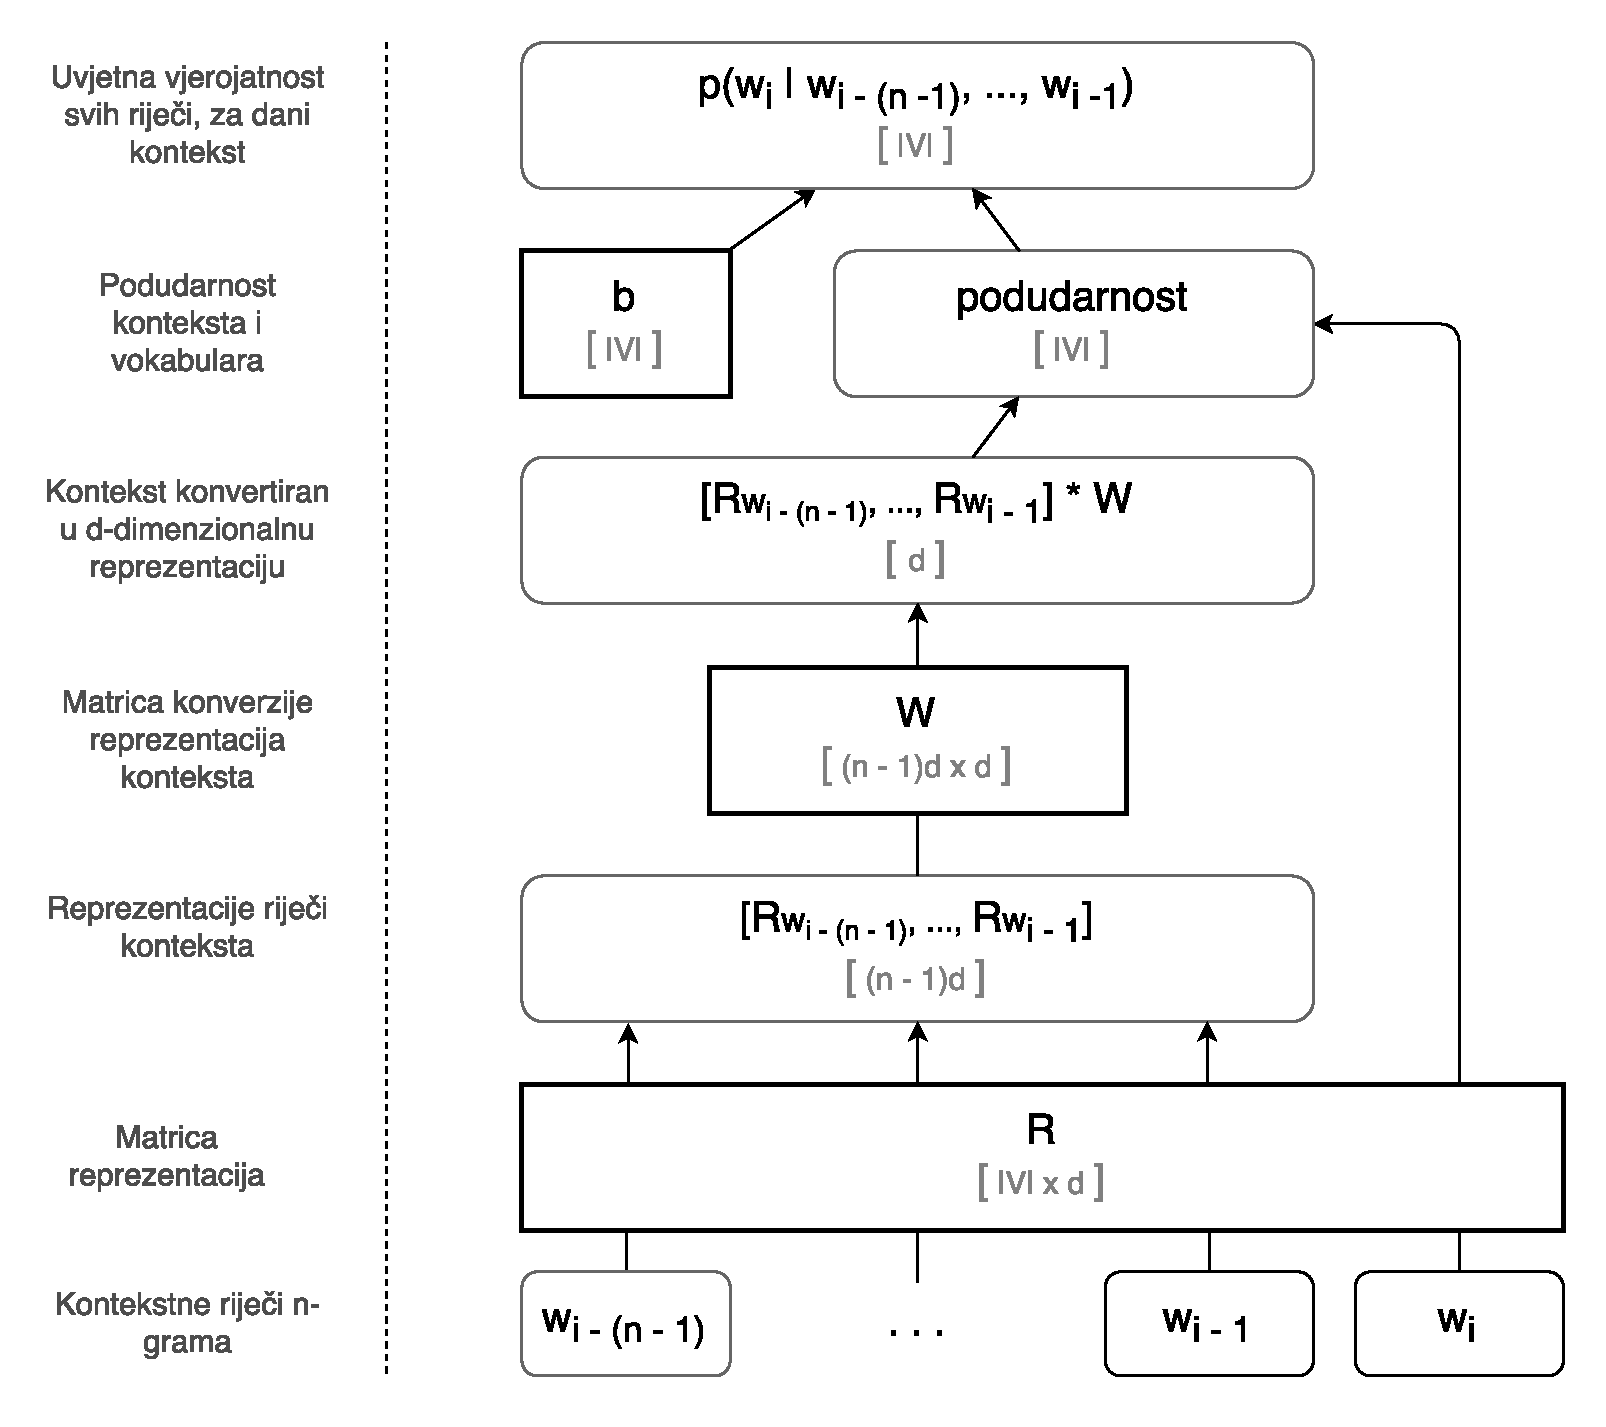
\includegraphics{fig/lbl.pdf}
\caption{Arhitektura log-bilinearnog jezičnog modela. Pravokutnici s debljim rubovima su parametri modela. Pravokutnici sa zaobljenim rubovima su podatci koji prolaze kroz model.}
\label{fig:lbl}
\end{figure}

\section{Učenje}

Log-linearni modeli poput \textit{softmax}-a se u pravilu treniraju iterativno, gradijentnim smanjenjem funkcije greške. Isti princip učenja primjenjiv je i na log-bilinearni model. Materijali na tu temu su široko dostupni, stoga ona neće biti razložena u ovom radu.

Specifičnost jezičnog log-bilinearnog modela je istovremeno učenje parametara linearne funkcije $W$ i $b$, te matrice reprezentacija vokabulara $R$. Gradijentno smanjenje greške s obzirom na matricu $R$ općenito je već spomenuta u poglavlju \ref{sec:nnet_grad}. U log-bilinearnom modelu dodatno je zanimljivo što se matrica $R$ koristi na dva mjesta u funkciji. Prvo za dobivanje reprezentacija konteksta, a potom za podudarnost reduciranog konteksta sa svim riječima vokabulara. S obzirom na dobro poznati problem "nestajućeg gradijenta" u treniranju neuronskih mreža, odnosno općenito slojevito definiranih modela, može se očekivati da gradijenti matrice $R$ budu osjetno veći s obzirom na konačni izračun podudarnosti. U tom slučaju učenje prilagođava matricu $R$ rezultatu kompozicije, što u teoriji može smanjiti kvalitetu učenja matrice kompozicije $W$ i reprezentacija $R$ koje doprinose boljim kompozicijama. Stoga je smisleno zapitati se bi li korištenje dviju matrica reprezentacija bilo prikladnije, iako i dalje vrijede protuargumenti navedeni u poglavlju \ref{sec:nnet_grad}. Zbog vremenskih ograničenja pokušaj učenja modela korištenjem dviju reprezentacijskih matrica nije iskušan. U radu CITAT korištena je samo jedna, a pošto su dobiveni rezultati  vrlo konkurentni drugim modelima, može se zaključiti učenje modela sa samo jednom matricom $R$ funkcionira dobro.

\section{Složenost modela}

Log-bilinearni model, kao i neuronska mreža, gradijentnim spustom smanjuje grešku procjene mjenjajući parametre modela (matricu preslikavanja, pristranosti). U tom smislu je zanimljivo usporediti broj parametara log-bilinearnog modela i neuronske mreže.

Matrica distribuiranih reprezentacija $R$ sadrži $|V| d$ parametara, matrica preslikavanja $W$ sadrži $(n - 1) d d$ parametara, a vektor pristranosti $d$ parametara. Sveukupno, log-bilinearni model sadrži $\left((n - 1) d + |V| + 1\right) d$ parametara. Memorijska složenost ovisi o dominantnom faktoru i stoga glasi $O(d |V|)$, što je $n$ puta manje od memorijske složenosti neuronske mreže. Isto tako, ta složenost ne ovisi o parametru $n$ (za smislene vrijednosti $n$), što znači da se veličina konteksta log-bilinearnog modela može povećavati bez da se znatno poveća memorijski zahtjevi modela.

Vremensku složenost treniranja i korištenja modela isto tako je teško procjeniti, kao i kod neuronske mreže. Trajanje treniranja modela svakako ovisi o broju parametara, pa je aproksimacija vremenske složenosti kao $O(d |V|)$ opravdana. Još jedna zanimljivost ovog modela je da je složenost korištenja modela vjerojatno niža od memorijske složenosti. Iz matematičke definicije modela vidljivo je da se reprezentacije dobivaju iz matrice $R$ naprosto indeksiranjem prikladnog retka te matrice, čak nije taj redak potrebno kopirati, što je vrlo jeftina operacija. Računske operacije pri korištenju modela se dešavaju u prostoru parametara koji ovisi samo o veličini reprezentacije $d$ i veličini konteksta $n$. Ne ovise o veličini vokabulara. Stoga korištenje modela (naspram treniranja) vrlo vjerojatno ima vremensku složenost $O(d n)$, što je puno manje od vremenske složenosti korištenja neuronske mreže, aproksimirane s $O(n d |V|)$.

\section{Implementacija}

Za implementacije neuronskih mreža dostupni su mnogi alati. Većina njih je visoko optimizirana kako bi što učinkovitije koristili dostupne računalne resurse. Višeprocesorska i višejezgrena računala koriste se za paralelizaciju treniranja mreže, a sve dostupnija je i podrška za treniranje mreža koristeći visoki stupanj paralelizma grafičkih procesora. Nadalje, alati često podržavaju definiciju mreže na visokom stupnju apstrakcije i automatizirani izračun gradijenata, što olakšava implementaciju i smanjuje količinu grešaka u programskom kodu.

U ovom radu za korištena je \textit{open-source} knjižnica Theano\footnote{http://deeplearning.net/software/theano/}, čije sučelje je dostupno za jezik Python\footnote{https://www.python.org/}. Odabrana je zbog fleksibilnosti definiranja modela (lako se koristi s visoke razine apstrakcije, ali omogućava i rad na nižim razinama), automatiziranog izračuna gradijenata i mogućnosti izvršvanja istog koda na centralnim i grafičkim procesorima.

\section{Implementacija}

Log-bilinearni model malo je manje uobičajen od unaprijednih neuronskih mreža. Nisu poznati alati koji bi omogućili definiranje takvog modela na visokoj razini apstrakcije dostupnoj za neuronske mreže, ali su alati za numeričku optimizaciju malo niže razine apstrakcije svejednako od velike koristi. Konkretno, postoji više komercijalnih i besplatnih alata koji omogućavaju simboličku definiciju log-bilinearnog modela, te automatizirani izračun gradijenata i optimizirani proces treniranja.

Kao i za model jezika temeljen na neuronskog mreži, za implementaciju log-bilinearnog modela korištena je knjižnica Theano. Knjižnica je korištena za automatsko izračunavanje gradijenta te optimalno treniranje modela na centralnim i grafičkim procesorima.

\chapter{Ograničeni Boltzmannov stroj}

U radu CITAT razmatra se i jezični model temeljen na ograničenom Boltzmannovom stroju (u nastavku "RBM", od engl. \textit{Restricted Boltzmann Machine}). RBM je generativni probabilistički model CITAT zanimljive formulacije, te ga stoga vrijedi spomenuti, iako je u spomenutom radu manje uspješan od log-bilinearnog modela.

RBM je dvoslojni probabilistički model. Prvi, vidljivi, sloj sadrži binarne ili mulitinomijalne varijable, dok drugi sloj predstavlja latentne varijable isključivo binarnog tipa. Vjerojatnost stanja cjelokupne mreže definirana je kao eksponencirana negativna energija modela, kao u Boltzmannovoj distribuciji, otkud dolazi ime.

\begin{equation}
\label{eq:rbm_p}
P(s) = \frac{\exp(-E(s))}{\sum_{s'}\exp(-E(s'))}
\end{equation}

Pri tome je vektor $s$ proizvoljno stanje svih neurona mreže, odnosno unija vidljivih neurona $v$ i skrivenih neurona $h$. Energija mreže je linearna funkcija stanja neurona. RBM je po definiciji potpuno spojeni bipartitni graf neurona vidljivog i skrivenog sloja. Energija je definirana na sljedeći način.

\[
E(s) = E(v, h) = - v W h^T  - v b_v - h b_h
\]

Pri tome je $W$ matrica težinskih veza među neuronima vidljivog i skrivenog sloja, $b_v$ pristranosti vidljivog sloja, a $b_h$ pristranosti skrivenog sloja.

Sličnost s već definiranim log-bilinearnim i \textit{softmax} modelom je očita. Što RBM čini specifičnim je to da su neuroni mreže probabilistički, a ne deterministički. Vjerojatnost binarne aktivacije vidljivog neurona $v$ (preuzimanja stanja $0$ ili $1$) u skladu s \ref{eq:rbm_p} je definirana kao funkcija energije.

\[
 P(v_i = 1) = \frac{1}{ 1 + e^{- ( W_i h^T + b_s)}} = \sigma( W_i h + b_{vi})
\]

Pri tome $W_i$ označava redak matrice koji odgovara vidlivom neuronu $v_i$. Može se primjetiti kako vjerojatnost aktivacije vidljivog neurona ovisi samo o stanjima skrivih, a ne o ostalim vidljivim neuronima. Kao što je spomenuto, neuroni su u RBMu organizirani u bipartitan graf, dakle veze među neuronima istog sloja ne postoje. Vjerojatnost aktivacije skrivenog neurona ima identičan izraz, s obzirom na vidljive neurone. Probabilistička aktivacija neurona specifično je svojstvo RBMova i modela temeljenih na RBMova koja ima snažno regularizacijsko djelovanje. Stoga su RBMovi često korišteni za pohlepono pred-treniranje slojeva dubokih neuronskih mreža CITAT, iako se rijetko koriste u konačnim mrežama jer deterministički neuroni uglavnom daju bolje rezultate CITAT. Detaljnije teoretsko i praktično razmatranje RBMa dostupno je u CITAT-Stamenković.

\section{RBM jezični model}

RBM je generativni probabilistički model, što znači da modelira vjerojatnosnu distribuciju pojavljivanja primjera i pripadnosti tog primjera nekoj klasi, u diskriminacijskoj primjeni. Za izradu jezičnog modela RBM ovakav model se može primjeniti za modeliranje distribucije \textit{n}-grama, odnosno uvjetnu vjerojatnost posljednje riječi \textit{n}-grama za dani konktekst od prethodnih ($n$ - 1) riječi. Da bi se došlo do izraza za vjerojatnost, potrebno je prvo definirati energiju.

\[
E(w_{i - (n - 1)}, ... , w_i, h) =  - d(w_{i - (n - 1)}, ... , w_i) (W h + b_v) - h b_h
\]

Na temelju energije može se definirati uvjetna vjerojatnost posljednje riječi \textit{n}-grama i stanja skrivenog sloja.

\[
P(w_i, h | w_{i - (n - 1)}, ... , w_{i - 1})
 = \frac{\exp(-E(w_{i - (n - 1)}, ... , w_i, h))}
  {\sum_{h'} \sum_w \exp(-E(w_{i - (n - 1)}, ... , w_{i - 1}, w, h'))}
\]

Konačno, marginalizacijom po svim mogućim stanjima skrivenog sloja može se izraziti uvjetna vjerojatnost posljednje riječi \textit{n}-grama.

\[
P(w_i | w_{i - (n - 1)}, ... , w_{i - 1})
 = \frac{\sum_h \exp(-E(w_{i - (n - 1)}, ... , w_i, h))}
  {\sum_{h'} \sum_w \exp(-E(w_{i - (n - 1)}, ... , w_{i - 1}, w, h'))}
\]

\section{Učenje}

Gradijentnu minimizacija funkcije greške  teško je izravno primjeniti zbog binarnih stohastičkih neurona. Kako bi se izračunali točni gradijenti greške, potrebno bi bilo evaluirati sve moguće konfiguracije binarnih neurona. Stoga se u praksi koristi algoritam "kontrastna divergencija", koji gradijentni spust aproksimira CITAT. Definicija algoritma i praktične implikacije izlaze izvan okvira ovog rada, detalji se mogu pronaći u mnogim dostupnim materijalima na temu, primjerice CITAT.

\section{Implementacija}

Grafički modeli sa stohastičkim varijablama kompleksniji su za treniranje od determinističkih modela. Razloga je više. Prvo, egzaktni izračun vjerojatnosti tipično podrazumijeva marginalizaciju po sivm mogućim stanjima skrivenog sloja. Iako se domišljatim trikom CITAT ovo može obavit u linearnom vremenu (s obzirom na broj neurona skrivenog sloja), izračun može biti numerički osjetljiv. Nadalje, treniranje i korištenje modela dobiva dodatno na računskoj složenosti korištenjem stohastičkih neurona, koji se oslanjaju na generatore nasumičnih brojeva. Što se tiče treniranja, parametre je potrebno podešavati "ručno" na temelju pseudo-gradijenata izračunatih kontrastnom divergencijom. Ovo otežava korištenje efikasnih numeričkih alata i implementaciju.

Unutar ovog rada jezični model baziran na RBMu implementran je korištenjem Theano knjižnice. Model je treniran algoritmom kontrastne divergencije. S obzirom na vremenska ograničenja, rezultirajuća implementacija je suboptimalna i komplicirana u odnosu na ostale modele u ovom radu. Provedeno je treniranje i vrednovanje ograničene uspješnosti. Iako je RBM pokazao najlošije rezultate u radu CITAT na kojem je ovaj baziran, moguće je da je implementacija RBMa ponuđena u ovom radu neispravna, uz to što je po definiciji osjetno sporija od drugih isprobanih metoda. S obzirom na kompleksnost ovog modela i poznato slabije rezultate, čini se da je praktično najmanje zanimljiv i isplativ od isprobanih rješenja.

\chapter{Vrednovanje}
\label{sec:eval}

\section{Metodologija}

Svrha jezičnog modela je ocjena sukladnosti neviđenog teksta i korpusa nad kojim je treniran. Za ocjenjivanje uspješnosti modela vrijede isti koncepti koji se primjenjuju u strojnom učenju općenjito. Ukratko, model je potrebno vrednovati korištenjem podataka koji su došli iz iste distribucije kao i podatci s kojima je model treniran, ali istovremeno oni moraju biti nezavisni. U skladu s tim, tipičan pristup vrenovanju je da se cjelokupni skup podataka dostupan za implementaciju modela podijeli da skup za treniranje, i skup za testiranje. Veličina ispitnog skupa ovisi o modelu, primjeni i količini dostupnih podataka. Pošto se jezični modeli tipično treniraju nad vrlo velikim korpusima, podataka u pravilu ima dovoljno. Stoga se za ispitni skup odvaja okvirno 5-10 posto svih podataka, dovoljno da bi ispitni skup imao sličnu distribuciju kao cijeli korpus, ali bez da se model zakine za previše podataka za učenje.

\section{Mjera uspješnosti jezičnog modela}

Za vrednovanje uspješnosti prediktivnih modela koriste se standardizirane mjere. Uobičajeno je za klasifikaciju koristiti mjeru točnosti predikcije nad ispitnim skupom. Točnost je udio primjera ispitnog skupa kojima je model dodjielio prikladnu oznaku klase. Za situacije kada svaka klasa nije podjednako zastupljena u skupu za treniranje, prikladnija je F mjera uspješnosti CITAT, koja stavlja jednaki naglasak na svaku klasu, bez obzira na njenu zastupljenost.

Navedene mjere nisu prikladne za ocjenu jezičnih modela zbog ambivalentnosti koja je jeziku inherentna. Za ilustraciju, konteksta \textit{"Znaš da volim..."} smisleno mogu nastaviti riječi \textit{"cirkus"}, \textit{"mrkvu"}, \textit{"skakati"} i brojne druge. Bilo bi stoga neispravno jezični model ocjeniti neuspješnim ako je kao nastavak predvidio riječ \textit{"automobile"}, a u ispitnom skupu je dati kontekst nastavljen s riječi \textit{"motocikle"}. Istovremeno, može se očekivati od modela da ipak neku zamjetnu vjerojatnnost za dani kontekst dodijeli i riječi \textit{"motocikle"}. Stoga se ocjenjuje upravo ta vjerojatnost.

Najčešće korištena mjera uspješnosti jezičnog modela je \textit{"perplexity"} (u prijevodu \textit{"zbrka"}, \textit{"zbunjenost"}). Matematička definicija mjere za distribuciju diskretne varjable slijedi.

\[
\mathcal{P} = b^{- \sum_x p(x) log_b q(x)}
\]

Pri tome je $p(x)$ istinska vjerojatnost pojavljivanja \textit{n}-grama $x$, $q(x)$ predikcija vjerojatnosti za $x$ od strane modela, $b$ baza logaritma (tipično se koriste $2$ ili baza prirodnog logaritma $e$), a $H(p)$ je entropija vjerojatnosne distribucije, mjera često korištena u teoriji informacije. Unutar ovog rada korištena je baza prirodnog logaritma $e$.

\[
\mathcal{P} = \exp\left(- \sum_x p(x) \ln q(x) \right)
\]

Kada se ova mjera koisti na skupu za testiranje u pravilu se pretpostavlja da je vjerojatnost primjera $p(x)$ jednaka udjelu tog primjera u skupu za testiranje, odnosno da je $p(x) = 1 - N_t$, gdje je $N_t$ broj primjera u testnom skupu.

\[
\mathcal{P} = \exp\left(- \sum_x \frac{1}{N_t} \ln q(x) \right)
\]

Konačni izraz za mjeru vrednovanja, koji koristi uvjetnu vjerojatnost pojavljivanja riječi, tada je definiran na sljedeći način.

\[
\mathcal{P} = \exp\left(- \frac{1}{N_t} \sum_{w_{i - (n - 1)}, ..., w_n}  \ln P(w_i | w_{i - (n - 1)}, ... , w_{i - 1}) \right)
\]

Ovako definirana mjera uspješnosti modela može se interpretirati na sljedeći način. Poželjno je da model primjer $w_{i - (n - 1)}, ..., w_n$ iz ispitnog skupa ocijeni sa što većom vjerojatnošću. Logaritam te vjerojatnosti ju preslikava u interval $(- \infty, 0)$. Uprosječen logaritam vjerojatnosti po svim primjerima ispitnog skupa naglašava niske vjerojatnosti, odnosno loše procjene modela. Eksponenciranjem negativnog prosjeka mjera se vraća iz logaritamskog u vjerojatnosni prostor. Konačna brojka stoga označava obrnutu prosječnu procjenu vjerojatnosti \textit{n}-grama modela, odnosno koliko je model "nesiguran" da riječ $w_n$ smisleno nastavlja kontekst $w_{i - (n - 1)}, ... , w_{i - 1}$. Dakle, dobar model ima malu mjeru \textit{perplexity}.

Potrebno je razmotriti i korištenje mjere \textit{perplexity} za usporedbu s modelima iz drugih radova. Generalno govoreći, izravnu usporedbu treba izbjegavati. Razlog tome je što mjera \textit{perplexity} jako ovisi o vokabularu korištenom za izgradnju jezičnog modela, kao i veličini skupa za treniranje i evaluaciju, odnosno podudarnosti distribucija tih dva skupa. Konkretno, korištenjem manjeg vokabulara (koji može biti naprosto posljedica drukčijeg pretprocesiranja teksta) moguće je na manjem, ali konzistentnom, korpusu postići vrlo niske rezultate mjere \textit{perplexity}. Ovo može navesti na krivi zaključak kako je dotični model bolji od nekog drugog modela treniranog na većem korpusu s većim vokabularom. U tom smislu je mjera \textit{perplexity} prikladna isključivo za usporedbu modela treniranih na istom korpusu s istim vokabolarom.

\section{Korpus}

Za vrednovanje jezičnih modela implementiranih u ovom radu koristiti će se korpus iz \textit{Microsoft Research Sentence Completion Challenge} CITAT (u nastavku MRSCC). Zadak u MRSCC je izgraditi jezični model koji za svaku od 1040 rečenica testnog skupa odabire točnu riječ koja rečenicu kompletira, između pet ponuđenih. Rečenice su sve uzete iz Sir Arthur Conan Doyle-ovog serijala o detektivu Sherlocku Holmesu. U svakoj rečenici je za jednu riječ osmišljeno četiri alternativne, koje su sintaktički ispravne, ali semantički neispravne. Primjer jedne rečenice i ponuđenih alternativa slijedi.

\begin{enumerate} 
\item{The king \textbf{landed} at him in amazement.}
\item{The king \textbf{rejoiced} at him in amazement.}
\item{The king \textbf{smiled} at him in amazement.}
\item{The king \textbf{knocked} at him in amazement.}
\item{The king \textbf{stared} at him in amazement.}
\end{enumerate}

U navedenom primjeru naviše smisla ima posljednja rečenica (\textit{"stared"}). Treća rečenica (\textit{"smiled"}) je donekle smislena, dok ostale osjetno manje. Upravo zbog toga što su niti jedan primjer nije sasvim besmisle je MRSCC zadatak vrlo zanimljiv. Čovjek koji dobro govori engleski jezik lako zadatak riješi s točnošću preko 90\%. Istovremeno je za računalo zadatak iznimno težak, jer se bazira na semantičkom povezivanju koncepata i tumačenju konteksta rečenice. U trenutku pisanja svi računalni jezični modeli na MRSCC testu postižu točnost ispod 60\% CITAT.

Za MRSCC je propisan i točno definiran korpus teksta nad kojim je dozvoljeno graditi model. Time se osigurava da sve implementacije imaju iste početne uvjete. Primjerice, nije dozvoljeno koristiti javno dostupne Google \textit{n}-grame CITAT, jer su oni pobrojani iz puno većeg korpusa teksta, koji možda čak čak obuhvaća rečenice iz skupa za testiranje. Propisani korpus se sastoji od 522 književna djela (pretežno romana) engleskog govornog područja iz istog vremenskog perioda u kojem je pisao Conan Doyle (19.\ stoljeće). Cijeli korpus sadrži oko 50 milijuna riječi, a preuzet je sa stranica Guttenberg projekta\footnote{https://www.gutenberg.org/}, gdje su korištena djela dostupna u cijelosti, bez legalnih restrikcija.

Unutar ovog rada jezični modeli su vrednovani primarno korištenjem mjere \textit{"perplexity"} na ispitnom skupu uzetom iz samog skupa za treniranje. Vrednovanje na MRSCC zadatku je sekundarno. Razlog je to što cijeli korpus of 50 milijuna riječi zahtjeva računalne resurse i vrijeme za treniranje koji za pisanje ovog diplomskog rada nisu dostupni. Moguće je implementirati modele koji se treniraju nad podskupom od 20 romana (od dostupnih 522), odnosno 1.8 (od dostupnih 50) milijuna riječi. Stoga je nemoguće rezultate testiranja uspoređivati sa rezultatima modela treniranih nad cijelim MRSCC korpusom, od primarnog interesa je realtivna usporedba različitih pristupa izgradnji jezičnih modela.

\section{Predprocesiranje i normalizacija teksta}

Korpus za treniranje dostupan je u obliku u kojem je obljavljen u sklopu Guttenberg projekta. Potrebno je pročistiti ga kako bi se dobio tekst prikladan za izgradnju jezičnog modela. Prvo su maknuta zaglavlja i ostali dodatci samog Guttenberg projekta, pošto oni nisu dio originalnog teksta. Brojevi pisani znamenkama se zamjenjuju posebnim tokenom. Potom se tekst dijeli na rečenice i riječi korištenjem knjižnice za procesiranje prirodnog jezika SpaCy\footnote{https://honnibal.github.io/spaCy/}. Rezultat su riječi grupirane u rečenice, pri čemu riječ sadržava samo slova, bez interpunkcije i praznina.

U svakom većem korpusu teksta je razdioba korištenja riječi slična. Mali broj riječi se koristi velik broj puta (to su tipično denominatori, zamjenice itd.), dio riječi je učestao ali ne brojan (često korištene imenice, glagoli i pridjevi), te je konačno velik broj riječi korišten samo nekoliko puta. Pošto računalna složenost svih jezičnih modela raste s veličinom vokabulara, tipično se riječi malog broja pojavljivanja ignoriraju, odnosno zamjenjuju jednim tokenom koji ih predstavlja sve. Osim smanjenja vokabulara, time se iz korpusa pročisti i dobar dio krivo napisanih riječi. Na korištenom podskupu MRSCC korpusa kriterij korištenja riječi je da se pojavila barem 5 puta, u barem 2 književna djela. Time je vokabular od preko 37 tisuća riječi smanjen na manje od 13 tisuća, skoro trostruko, a da pri tome odbačene riječi predstavljaju samo 4.5 posto korpusa.

Osim odbacivanja malo korištenih riječi, tekst se često normalizira po pitanju morfološke varijacije. Za velik broj primjena jezičnih modela nije bitno primjerice glagosko vrijeme, stoga je poželjno da se, u domeni engleskog jezika, riječi \textit{"walk"}, \textit{"walks"} i \textit{"walked"} tretiraju kao ista riječ. To povećava broj primjera u kojem jezični model vidi glagol \textit{"walk"}, što omogućava bolju generalizaciju. Naravno, postoje primjene jezičnih modela (automatsko prevođenje, provjera ispravnosti teksta) u kojima su distinkcije po glagolskom vremenu bitne. Unutar ovog rada pretpostavljamo primjenu koja je u skladu s MRSCC. Povezivanje semantike riječi bitnije je od morfološke ispravnosti jezičnod modela.

 Za takvu primjenu potrebno je obaviti normalizaciju riječi. Tipični pristupi za normalizaciju teksta su lematizacija \engl{lemmatisation} i skraćivanje riječi na korijen \engl{stemming}. Lematizacija riječ svodi na morfološki neutralan oblik iste vrste (pridjev "sjajan" se ne svodi na imenicu "sjaj" iz koje je izveden), dok skraćivanje na korijen primjenom infleksijskih pravila rezultira grubljom normalizacijom (pridjev "sjajan" biti će svedeno na korijen "sjaj"). Dodatno, ponekad se koristi još agresivniji oblik skraćivanja gdje se od svake riječi uzima samo prvih $k$ slova. Prednost ovog pristupa je da je vrlo jednostavan za implementaciju i dobro radi u jezicima s malim brojem složenih riječi, poput engleskog.

 Unutar ovog rada isprobano je korištenje lematizatora knjižnice SpaCy i skraćivanje na prvih $k$ slova, pri čemu je parametar $k$ optimiziran. Inicijalno testiranje na MRSCC zadatku, korištenjem 4-grama, je pokazalo da skraćivanje na prva $4$ slova daje najbolje rezultate. Iako se može činiti kao pre-agresivan oblik normalizacije, u skladu je s Google-ovim eksperimentima\footnote{https://www.youtube.com/watch?v=nU8DcBF-qo4}. Korištenjem skraćivanja na prva 4 slova vokabular od oko 38 tisuća riječi je sveden na nešto manje od 10 tisuća prefiksa. Nakon što se primjeni odbacivanje riječi koje su se pojavile manje od pet puta ili u samo jednom romanu MRSCC korpusa, ostaje tek 5133 prefiksa. Istovremeno, manje riječi se odbacuje, iskorištenost korpusa postaje preko 99 posto. 


\section{Rezultati}

U konačnici su vrednovana četiri modela. Prva da se baziraju na prebrojavanju \textit{n}-grama uz aditivno i Kneser-Ney zaglađivanje. Treći model je neuronska mreža, a posljednji je log-bilinearni model.

Podatci za treniranje su prvih dvadeset romana iz MRSCC korpusa, koji sveukupno sadrže oko 1.8 milijun riječi. Konačni broj \textit{n}-grama varira s obzirom na parametar \textit{n}, jer se \textit{n}-grami generiraju iz rečenice, nikad ne sadrže riječi iz dvije susjedne rečenice. Iz skupa za treniranje je tisuću \textit{n}-grama izdvojeno za validaciju tijekom treniranja, a pet posto (oko 90 tisuća \textit{n}-grama) za konačno vrednovanje.

Za modele zaglađenog prebrojavanja se korištenjem validacijskog skupa optimiraju parametri zaglađivanja \textit{lambda} (kod aditivnog zaglađivanja) i \textit{delta} (kod Kneser-Ney zaglađivanja). Za neuronsku mrežu i log-bilinearni model su hiperparametri modela (L2 regularizacija, veličina mini-grupe) odabrani u skladu s postojećim eksperimentima CITAT, nisu optimirani. Isto vrijedi i za parametre gradijentnog spusta, koristi se naime RMSprop CITAT, koji veličinu gradijentnog pomaka prilagođava automatski, te rijetko zahtjeva eksplicitno podešavanje. Validacijski skup je korišten za određivanje trajanja treniranja. Model se trenira sve dok mjera \textit{perplexity} na validacijskom skupu pada za barem 1 u posljednje tri epohe.

\subsection{Vrednovanje mjerom \textit{perplexity}}

Tablica \ref{tbl:eval_perplexity} prikazuje rezultate treniranih modela na skupu za testiranje, vrednovanjem mjerom \textit{perplexity}.

\begin{table}[htb]
\caption{Rezultati vrednovanja jezičnih modela mjerom \textit{perplexity} za \textit{n}-grame zaglađene aditivno i Kneser-Ney metodom, neuronsku mrežu i log-bilinearni model, po stupcima za različite vrijednosti parametra $n$.}
\label{tbl:eval_perplexity}
\centering
\begin{tabular}{lccc}
\toprule
 & \multicolumn{3}{c}{Parametar \textit{n}} \\
\cmidrule(r){2-4}
Model & 3 & 4 & 5 \\
\midrule
Additivno &  305 & 1182 & 2680 \\
Kneser-Ney & 72 & 121 & 204 \\
Neuronska mreža & 117 & 114 & 113 \\
Log-biliner & 102 & 98 & 98 \\
\bottomrule
\end{tabular}
\end{table}

Najbolje rezultate daje jezični model baziran na prebrojavanju i zaglađivanju Kneser-Ney metodom. Model baziran na aditivnom zaglađivanju daje najgore rezultate, što je u skladu s očekivanjem. Vidljivo je kako rezultati modela baziranih na prebrojavanju padaju sa povećanjem parametra $n$, odnosno veličinom konteksta. Ovo je izravno povezano s već razmatranom posljedicom povećanog konteksta, u smislu sve veće rijetkosti pojavljivanja duljih \textit{n}-grama u ograničenom korpusu. Korištenjem cijelog MRSCC korpusa bi rezultati za dulje kontekste ($n \in \{5, 6\}$) svakako bili osjetno bolji, čak i bolji od rezultata kraćih ($n \in \{3, 4\}$) CITAT.

Rezultati jezičnih modela baziranih na neuronskoj mreži i log-bilinearnom modelu daju dobre rezultate. Poznato je da među ta dva modela log-bilinerani radi bolje CITAT, što pokazuju i pokusi izvedeni u ovom radu. Zanimljiv aspekt ovih modela je kako njihove performanse rastu povećanjem konteksta. Razlog tomu je najvjerojatnije to što se distribuirane reprezentacije riječi u tim modelima računaju na temelju svih riječi u kontekstu. Stoga dulji kontekst modelu daje više informacije o međusobnoj sličnosti riječi te je učenje reprezentacija kvalitetnije. Istovremeno, za razliku od modela baziranih na prebrojavanju, neuronska mreža i log-bilinearni model su manje osjetljivi na rjetkost pojavljivanja duljeg konteksta, što izravno proizlazi iz sposobnosti modela za semantički slične riječi izluče slične reprezentacije.

Pitanje se postavlja zašto s obzirom na sve njihove prednosti, neuronska mreža i log-bilinearni model daju lošije rezultate od modela zaglađenog Kneser-Ney metodom. Razlog tomu je vrlo malen vokabular korišten za usporedbu dotičnih modela. Korištenje vrlo malog podskupa MRSCC korpusa, uz skraćivanje na prva četiri slova, rezultira iznimno malim vokabularom. Pošto su metode bazirane na prebrojavanju osjetljivije na veličinu vokabulara (jer ne koriste distribuirane reprezentacije), korištenjem većeg vokabulara za očekivati je da log-bilinearni model postigne bolje rezultate, u skladu s postojećim eksperimentima CITAT. Bitno je prisjetiti se ranije napomene kako dobiveni rezultati nisu prikladni za usporedbu s rezultatima iz drugih radova zbog korištenja različitog korpusa (podskup MRSCC korpusa naspram cijelog) i smanjenog vokabulara.

\subsection{Uspješnost modela na MRSCC zadatku}

Modeli su vrednovani i na konkretnom MRSCC zadatku odabira semantički točne riječi u rečenici, od pet ponuđenih. Mjera vrednovanja je udio točnih odabira na skupu od 1040 rečenica. Važno je napomenuti kako su rezultati koji slijede predviđeni za relativnu usporedbu korištenih modela. Usporedba s rezultatima iz drugih radova nije smislena jer je u ovom radu zbog vremenskih ograničenja korišten tek mali podskup MRSCC korpusa. Tablica \ref{tbl:eval_mrscc} prikazuje dobivene rezultate.

\begin{table}[htb]
\caption{Rezultati uspješnosti jezičnih modela na MRSCC zadatku.}
\label{tbl:eval_mrscc}
\centering
\begin{tabular}{lccc}
\toprule
 & \multicolumn{3}{c}{Parametar \textit{n}} \\
\cmidrule(r){2-4}
Model & 3 & 4 & 5 \\
\midrule
Additivno &  0.19 & 0.19 & 0.19 \\
Kneser-Ney & 0.27 & 0.27 & 0.24 \\
Neuronska mreža & 0.23 & 0.23 & 0.22 \\
Log-biliner & 0.25 & 0.27 & 0.27 \\
\bottomrule
\end{tabular}
\end{table}

Rezultati na MRSCC zadatku su u skladu s rezultatima korištenjem mjere \textit{perplexity}. Prebrojavanje \textit{n}-grama korištenjem aditivnog zaglađivanja daju najlošije rezultate (jednake uspješnosti nasumičnog odabira), dok prebrojavanje korištenjem zaglađivanja Kneser-Ney i log-bilinearni model daju bolje, približno jednake rezultate. I dalje je vidljivo kako modeli bazirani na prebrojavanju rade lošije kada je kontekst dulji, a log-bilinearni model bolje. Neuronska mreža konzistentno daje osrednje rezultate.

U radu unutar kojeg su se jezični modeli trenirali korištenjem cijelog MRSCC korupsa, najbolji rezultat postignut je korištenjem log-bilinearnog modela treniranog nad 10-gramima, prijavljena je 0.547 uspješnost (najbolja poznata u trenutku pisanja ovog rada). U istom radu model baziran na zaglađenom prebrojavanju \textit{n}-grama postiže 0.391 usješnost, korištenjem 4-grama. Čini se stoga da je log-bilinearni model generalno bolji, ali valja uzeti u obzir i trošak treniranja tavog modela.

\subsection{Trajanje treniranja}

Neuronske mreže i log-bilinearni model treniraju se iterativnom metodom gradijentnog smanjenja greške. Za velike modele (modele koji imaju velik broj slobodnih parametara) i velike skupove podataka za treniranje, učenje modela može zahtjevati veliku količnu vremena. Stoga je unutar ovog rada testirano i vrijeme potrebno za treniranje dotičnih modela. Modeli bazirani na prebrojavanju zahtjevaju samo jedan prolazak kroz \textit{n}-grame skupa za treniranje, i malu količinu dodatne analize. U pravilu treniranje i na slabijim modernim centralnim procesorima traje tek nekoliko minuta. Modeli bazirani na iterativnom smanjenju greške kompleksnijim algoritmima analiziraju skup za treniranje kroz veći broj iteracija (u ovom radu prosječno tridesetak iteracija). Stoga su trenirani na snažnom modernom centralnom procesoru\footnote{Intel i7-4720, 2.6GHz, 4 fizičke jezgre, 8-dretvi, 16GB RAM} (CPU), i na modernom grafičkom procesoru srednje klase\footnote{nVidia GeForce GTX 960M, 4GB RAM, 640 programabilnih CUDA jezgri} (GPU). Trajanje treniranja iterativnih modela prikazano je u tablici \ref{tbl:eval_time}. Bitno je napomenuti kako vremena treniranja ovise o mnogim čimbenicima kao što su optimalnost implementacije, kriterij zaustavljanja iterativnog treniranja, veličina minigrupe pri iterativnom treniranju, tip gradijentnog spusta koji se koristi itd. Stoga navedena vremena treba tumačiti kao vrlo okvirna, navedena su samo radi međusobne usporedbe.

\begin{table}[htb]
\caption{Trajanje treniranja modela, izraženo u SAT:MINUTE obliku.}
\label{tbl:eval_time}
\centering
\begin{tabular}{lccc}
\toprule
 & \multicolumn{3}{c}{Parametar \textit{n}} \\
\cmidrule(r){2-4}
Model & 3 & 4 & 5 \\
\midrule
Prebrojavanje \textit{n}-grama CPU &  0:01 & 0:01 & 0.01 \\
Neuronska mreža, GPU & 1:47 & 2:15 & 2:17 \\
Neuronska mreža, CPU & 13.38 & 13:52 & 14.20 \\
Log-bilinear GPU & 0:49 & 0:48 & 0:46 \\
Log-bilinear CPU & 8:07 & 8:01 & 6:56 \\
\bottomrule
\end{tabular}
\end{table}


Vidljivo je kako je vrijeme trajanja treniranja modela koji se baziraju na prebrojavanju neusporedivo kraće od treniranja neuronskih mreža i log-bilinearnog modela. Uzme li se u obzir da model koji koristi zaglađivanje Kneser-Ney metodom postiže vrlo dobre rezultate, lošije ali usporedive s rezultatima log-bilinearnog modela, taj model ostaje kompetitivan u situacijama gdje su računalni resursi ili vrijeme treniranja ograničeni. Nadalje, vidljive su ogromne razlike između vremena treniranja korištenjem centralnog odnosno grafičkog procesora. Pri tome je bitno uzeti u obzir i to da je korišten CPU visoke klase (u vrijeme pisanja rada), a korišteni GPU više-srednje klase. Usporeba vrhunskih centralnih i grafičkih procesora rezultirala bi još većom disproporcijom.

Zanimljivo je kako kod log-bilinearnog modela kraći kontekst rezultira sporijim treniranjem. Razlog tome je povećanje broja \textit{n}-grama kada se koristi kraći kontekst, što je posljedica toga da se \textit{n}-grami generiraju iz rečenica, bez preklapanja, što rezultira s $N - n + 1$ \textit{n}-gramom po rečenici, gdje $N$ označava broj riječi u rečenici. Tako se iz istog korpusa rečenica generira čak 4\% više trigrama nego 4-grama. Istovremeno, dodatne računske operacije potrebne za treniranje korištenjem duljeg konteksta imaju manji utjecaj zbog visokog paralelizma računanja da grafičkim karticama.

\chapter{Zaključak}

U ovom diplomskom radu vrednovani su jezični modeli izgrađeni korištenjem tri bitno različita pristupa. Prvi pristup, koji se već dugo koristi, bazira se na prebrojavanju \textit{n}-grama. Drugi pristup bazira se na neuronskoj mreži definiranoj kao klasifikator riječi koja slijedi proizvoljnom kontekstu prethodnih riječi. Treći pristup je najnoviji, bazira se na log-bilinearnom modelu koji ima znatno manji broj parametara od neuronske mreže.

Vrednovanje navedenih modela korištenjem podskupa korpusa \textit{Microsoft Research Sentence Completion Challenge} pokazala je kako najbolje rezultate daju model baziran na prebrojavanju i zaglađivanju Kneser-Ney metodom, i log-bilinearni model. Pri tome je pokazano da na manjem korpusu prebrojavanje daje nešto bolje rezultate, dok ispitivanja u drugim radovima pokazuju da na većem korpusu log-bilinearni model daje najbolje rezultate. Ispitano je i vrijeme potrebno za treniranje svih korištenih modela, pri čemu se pokazalo da je treniranje modela baziranih na prebrojavanju neusporedivo brže od treniranja neuronske mreže i log-bilinearnog modela. U tom smislu su modeli bazirani na prebrojavanju i dalje primjenjivi, bez obzira na relativno dugu povijest korištenja (prva implementacija je bila 1995.\ godine).

U napretku jezičnih tehnologija, poput prepoznavanja govora i automatiziranog prevođenja, jezični modeli imaju ključnu ulogu. Uz to oni nisu ograničeni samo na tu primjenu, mogu se koristiti za analizu i klasifikaciju teksta, detekciju grešaka u tekstu i za mnoge druge zadatke. Stoga je za očekivati da će se intenzivno istraživanje i razvoj ovog područja nastaviti. Trenutno je u području strojnog učenja i izadi prediktivnih modela snažan trend korištenja dubokih i konvolucijskih neuronskih mreža. Već postoje radovi koji primjenom ovih tehnika grade još sposobnije jezične modele. Njihova sposobnost prepoznavanja semantičkih uzoraka u tekstu se polako ali neosporivo približava ljudskoj. U tom smislu su jezični modeli jedna od krucijalnih komponenata izgradnje strojeva čija bi "inteligencija" bila usporediva s ljudskom.

\bibliography{literatura}
\bibliographystyle{fer}

\chapter{Sažetak}

\end{document}
